
%----------------------------------------------------------------------------------------
%	CHAP introduction
%----------------------------------------------------------------------------------------

\chapterimage{blue-chapter-head_4-reduced.pdf} % Chapter heading image

\chapter{Tables}\label{chap:Tables}
\section{Overview}
Before you start an analysis, you will need to define Table nodes that represent the data files needed in the analysis. MetaR explicitly models files that contain tables of data. This is done so that you can easily refer to these tables, without having to remember where the original file is located on your computer. 

\noindent In this Chapter, you will learn how to 
\begin{enumerate}
	\item define a MetaR table,
	\item  adjust the types of the columns of the data described in the file,
	\item annotate a table with groups,
	\item link groups in column group usage.
\end{enumerate}

\section{Create a Table}\label{sec:CreateATable}\index{Create a Table}
To create a Table, right-click on a model in the project tab and select \menu{right-click > New > o.c.metar.tables > Table}. This will create an empty table, as shown in Figure~\ref{fig:NewTable}. Tables have a \texttt{name}, a \texttt{pathToResolve} attribute and a list of columns. The following paragraphs describe these attributes.
\paragraph{name}
The table name is set automatically from the path when you use the file selection button. You can change the name to match your analysis needs and make it easier to remember what is in the table.
\paragraph{File Path (pathToResolve)}
This attribute contains a path to the TSV file that you wish to analyze. The path may contain references to path variables that will be automatically resolved before MetaR attempts to load table information from the path. Path variable references can be written as \texttt{\${a.b.c}/data/file.tsv}. Such a reference will require you to define the a.b.c path variable name and associate it with a value on each machine where the table will be used. You can define path variables with the Preferences/Settings MPS menu (\menu{MPS > Preferences> PathVariables} on Mac, \menu{MPS > Settings > PathVariables} on PC).

\paragraph{Columns}
Columns is an attribute that presents the list of columns identified in the TSV file. Each column has a name, a type, and may be annotated with a set of column groups (see Section~\ref{sec:ColumnGroups} for details about column groups).
MetaR supports the following column types, which map to the R data types:
\begin{enumerate}
	\item \textbf{Numeric}. Any number. Technically, can be a floating number or an integer.
	\item \textbf{String}. A string of characters.
	\item \textbf{Boolean}. A type that can only have two values: \texttt{true} or \texttt{false}.
	\item \textbf{Category}. A type that can take only a limited number of values (e.g., \{\texttt{RED}, \texttt{GREEN}, \texttt{BLUE}\} would be a category with these values, (\texttt{RED}, \texttt{GREEN} and \texttt{BLUE} in our example).
\end{enumerate}
These types are automatically determined from the data in the table file. However, in case the automatic algorithm failed for a table, you can change the types manually. To do this, put the cursor over the name of the type in the column section, and use auto-completion in the inspector to change to the desired type.
 
\begin{SCfigure}
  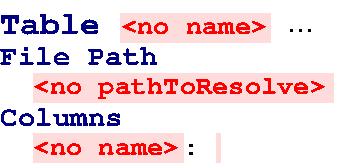
\includegraphics[width=\figWidthTiny]{figures/NewTable.pdf}
  \caption[New Table.]{\textbf{New Table.} This figure presents a freshly created Table AST Root node. You can use the button located to the right, after the <no name> red label (\keys{...}), to open a file selection dialog. Use this dialog to locate a TSV file to configure this table.}\label{fig:NewTable}
\end{SCfigure}

Figure~\ref{fig:ExampleTable} presents a MetaR table annotated with groups. \index{Example}

\begin{figure}[h!tbp]
  \centering
  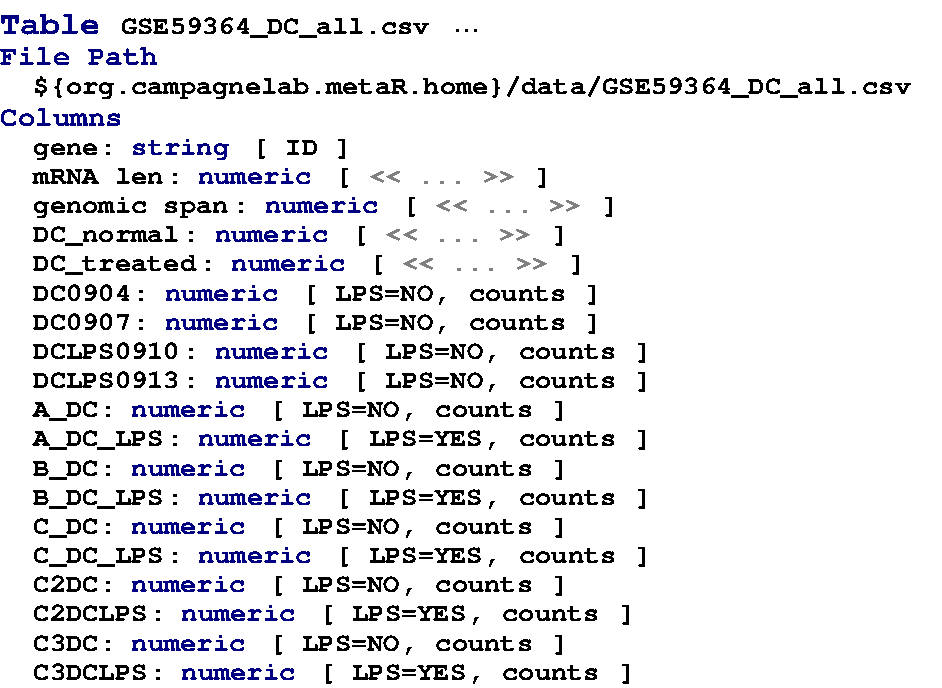
\includegraphics[width=\figWidthWide]{figures/ExampleTable.pdf}
\caption[Example Table.]{\textbf{Example Table.} The figure presents an example table annotated with groups.}
\label{fig:ExampleTable}
\end{figure}


\section{Column Groups Container}\label{sec:ColumnGroupContainer}\index{Column Groups Container}
Column Groups Containers are used to define column groups and annotate these groups with group usages.
To create a new Column Group Container, right-click on a model and select \menu{New > o.c.tables.ColumnGroupContainer}. This will create the empty container shown in Figure~\ref{fig:NewColumnGroupContainer}. You need and should have only one container per model. The container will hold the groups and group usages that you need across the MetaR Tables defined in the model.
\begin{SCfigure}
  \centering
  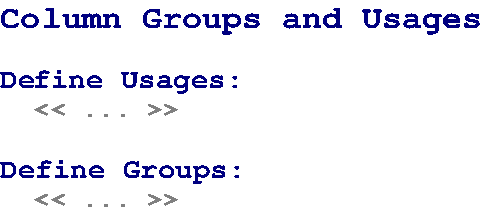
\includegraphics[width=\figWidthNarrow]{figures/NewColumnGroupContainer.pdf}
\caption[Empty Column Group Container.]{\textbf{Empty Column Group Container.} Use a column group container to define column groups and associated group usages. Place the cursor over the \mpsplaceholder{} symbol and press \keys{\return} to add a new group or group usage. Name the group or usage immediately after creating it.}
\label{fig:NewColumnGroupContainer}
\end{SCfigure}

\section{Column Groups}\index{Column Groups}\label{sec:ColumnGroups}
Column Groups can be defined by pressing \keys{\return} either on top of the \mpsplaceholder{} (immediately below \texttt{Define Groups:}), when the list of groups is empty, or with the cursor immediately before the name of an existing group. Each group has a name and an optional set of group usages. Figure~\ref{fig:NewGroup} presents a new column group (group for short).

\begin{SCfigure}
  \centering
  
\includegraphics[width=\figWidthNarrow]{figures/NewGroup.pdf}
\caption[New Group.]{\textbf{New Group.} You should name a new group immediately after creating it.}
\label{fig:NewGroup}
\end{SCfigure}

\paragraph{name} The name of the group is a string that should mean something in the context of your analysis. Some MetaR analysis statements require specific group names to be defined in a model container and referenced in an input table. Other groups will be created by you with meaningful names to help identify columns that have certain properties, so that you can refer to them collectively by the group name. 

\paragraph{used for}
Column groups can be annotated with a set of group usages. You can enter references to usages already defined in the column group container following the \texttt{used for} keyword shown in Figure~\ref{fig:NewGroup}. Press \keys{\enter} on the \mpsplaceholder{} to insert the first group usage. Make sure the usage is defined (its name should be visible in the \texttt{Define Usages:} section of the container (see Section~\ref{sec:ColumnGroupUsage} to lean how to create a new Group Usage). You can bind a group usage reference to a Group usage by using auto-completion (\keys{\ctrl+\space} to locate the name, then pressing \keys{\enter} to accept one completion choice), or by typing the name of the group usage directly (note that group usage names are case sensitive).

\begin{remark}
	Pressing \keys{\return} before \texttt{<no name>} will not have the desired effect if you have not yet named a group. Make sure you name groups immediately after you create them. 
\end{remark}

 
\section{Column Group Usage}\label{sec:ColumnGroupUsage}
A Column Group Usage can be defined by pressing \keys{\return} either on top of the \mpsplaceholder{} (immediately below \texttt{Define Usages:}), when the list of group usages is empty, or with the cursor immediately before the name of an existing group usage. When the list already contains one or more group usages, you can add more by placing the cursor over a group usage name and pressing \keys{\enter}. Keep pressing \keys{\enter} to add more empty group usages.

\section{Example Column Group Container}\index{Example}

\begin{SCfigure}
  \centering
  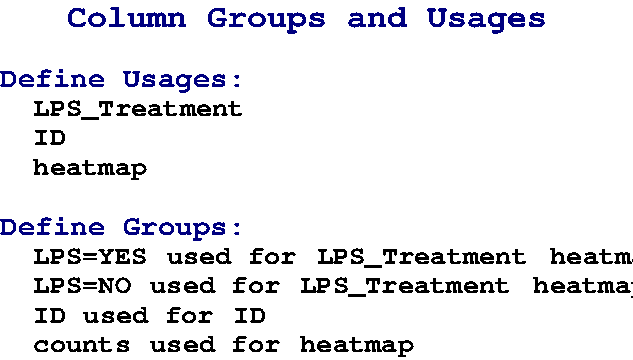
\includegraphics[width=\figWidthNarrow]{figures/ExampleGroupContainer.pdf}
\caption[Example Group Container.]{\textbf{Example Group Container.} This example presents a container with several groups and group usages.}
\label{fig:ExampleGroupContainer}
\end{SCfigure}

Figure~\ref{fig:ExampleGroupContainer} presents an example of a configured Column Group Container. This container defines two groups \texttt{LPS=yes} and \texttt{LPS=no}, which can be used to annotate Table columns that contain data about gene expression of samples treated with LPS or not.  The group usage \texttt{LPS\_Treatment} is associated to both groups to indicate that they belong together and are two kinds of treatment.


\section{Column Groups from a Table}\index{Column Groups Table}\label{sec:ColumnGroupsTable}
An alternative way to automatically create Column Groups and attach them to Columns at the same time is to use a so-called \texttt{annotation table}. These tables are normal Table nodes (created as specified \ref{sec:CreateATable}) with a special structure and content. When created, MetaR is able to recognize them and allows the user to use these tables to annotate other tables. 

The structure of an annotation table requires the following two columns: 
\begin{itemize}
\item \textit{SampleID}: values of this column are sample names
\item \textit{Groups}: values of this column are comma-separated lists of group names
\end{itemize}
\begin{SCfigure}
  \centering
  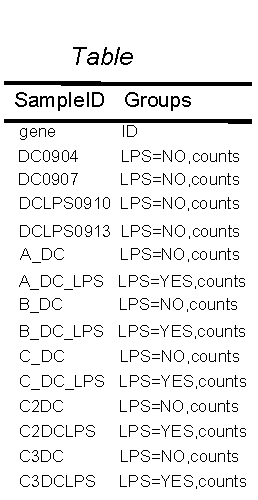
\includegraphics[width=\figWidthTiny]{figures/AnnotationTableSample.pdf}
\caption[Content of a Sample Annotation Table]{\textbf{Content of a Sample Annotation Table} The \texttt{SampleID} column provides the name of the column to which the groups should be assigned. The \texttt{Groups} column provides the names of the groups, separated by a comma, which will be assigned to the column identified by \texttt{SampleID}.}
\label{fig:AnnotateTableSample}
\end{SCfigure}


\noindent{}When annotation tables are available in the current model, the user can
\begin{enumerate}
\item  open the Table to annotate 
\item use the "Use Column Groups From Table: <table name>" intention (\intentionLightBulb) when the cursor is on top of the \texttt{Table} node
\end{enumerate}
This way, Sample IDs are matched with the column names and the groups listed in the same row are attached to the corresponding \texttt{Column}. In addition, if the groups are not defined in the \texttt{ColumnGroupContainer}, they are created in the annotation process. The \texttt{Column\allowbreak{}Group\allowbreak{}Container} is also created if it does not exist.


To see how this intention works in practice, we will create the same groups shown in Figure~\ref{fig:ExampleTable} using an annotation table. To do that, we firstly need to create a TSV file with the content shown in Figure~\ref{fig:AnnotateTableSample}. The next step is to load this table in a Table node (Figure~\ref{fig:NewAnnotationTable}).  Finally, we invoke the ``Use Column Groups From Table: Annotation\allowbreak{}Table\allowbreak{}For\allowbreak{}GSE59364\_DC\_all.cvs'' intention as shown in Figure~\ref{fig:AnnotateTableIntention} to apply the group names from the table to the destination Table. These steps will result in exactly the same annotated table shown in Figure~\ref{fig:ExampleTable}.

 
\begin{figure}[h!tbp]
  \centering
  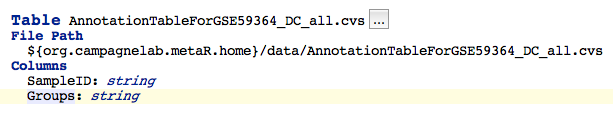
\includegraphics[width=\figWidthWide]{figures/AnnotationTable.png}
\caption[Table with Samples and Groups]{\textbf{Table with Samples and Groups.} An annotation table loaded as Table node.}
\label{fig:NewAnnotationTable}
\end{figure}


\begin{figure}[h!tbp]
  \centering
  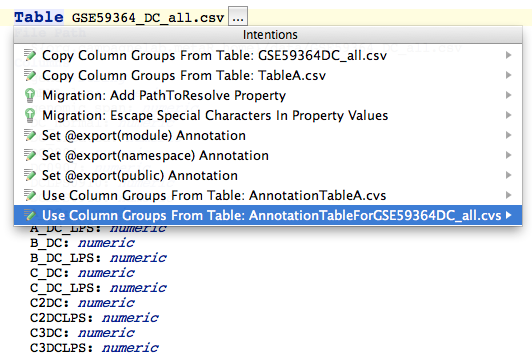
\includegraphics[width=\figWidthWide]{figures/AnnotateTableIntention.png}
\caption[Intention to Annotate a Table using another Table]{\textbf{Intention to Annotate a Table using another Table} }
\label{fig:AnnotateTableIntention}
\end{figure}

\section{Column Group Annotations}\index{Column Group Annotations}\index{New in MetaR 1.3}\label{sec:ColumnGroupAnnotations}
Sometimes, a covariate has different values for different samples (know as "continuous covariate"). This kind of covariate is very frequent when building linear models (see Chapter ~\ref{chap:EdgeR} and \ref{chap:LimmaVoom}). 

In this case, instead of creating a Column Group for each possible value of the covariate, MetaR offers the capability to use values coming from a selected column of a special type of table called Covariate Table.  A covariate table is a normal \texttt{Table} node in metaR with the following characteristics:
\begin{enumerate}
\item a column annotated with a group called "sample-key": 
\item values of this key column must match the sample names 
\item one or more additional columns from which covariate values are extracted 
\end{enumerate}
Figure~\ref{fig:CovariateTable} shows a simple covariate table.

\begin{figure}[h!tbp]
  \centering
  
\includegraphics[width=\figWidthWide]{figures/CovariateTable.pdf}
\caption[Covariate Table]{\textbf{Sample Covariate Table.} A covariate table must have a column annotated with the \texttt{sample-key} group, whose values are the sample names of the table that will be annotated with the Covariate table. The other columns hold the values that will be associated to each sample when they are selected.}
\label{fig:CovariateTable}
\end{figure}

A covariate table can be associated to a column group by pressing \keys{\lbrack} at the end of the group in the editor or by using the intention shown in Figure~\ref{fig:AddCovariateTable}.  The annotation added to the group allows to refer a covariate table in the current model and then select a column from that table with the covariate values (Figure~\ref{fig:GroupAnnotation}).

\begin{figure}
\centering
  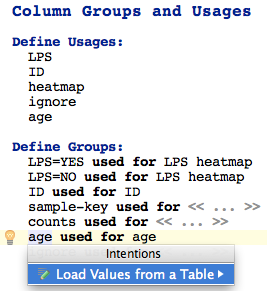
\includegraphics[width=\figWidthTiny]{figures/IntentionForAddingCovariateTable.png}
\caption[Intention to add a Covariate Table]{\textbf{Intention to Add a Covariate Table} }
\label{fig:AddCovariateTable}
\end{figure}

\begin{figure}
\centering
  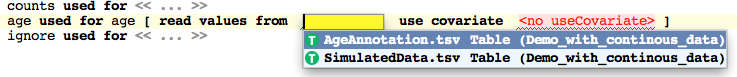
\includegraphics[width=\figWidthWide]{figures/GroupAnnotation.png}
\caption[Column Group Annotation]{\textbf{Column Group Annotation} Using auto-completion (\keys{\ctrl+\space} in the \texttt{no table} field, all the tables matching the covariate requirements are proposed. Once selected, a similar action can be used in the  \texttt{no useCovariate} field to select a column from that table. Values from that column are matched with the samples when a statement needs to build a linear model.}
\label{fig:GroupAnnotation}
\end{figure}

\section{Table Viewer Tool}\label{sec:TableViewerTool}\index{Table Viewer Tool}\index{New in MetaR 1.3}
\begin{remark}
The TableViewer Tool was introduced in MetaR version 1.3.
\end{remark}

The content of a Table can be inspected with the Table Viewer Tool distributed with MetaR. The tool adds to the MPS interface the capabilities to load the table's content and show it in a graphical context.
Wherever a table name appears (in a Table node or in an Analysis script, see Chapter~\ref{chap:Analyses}), the tool can be opened to see the rows and columns of that table along with their values. Figure~\ref{fig:ActivateTableViewer} shows how to activate the tool on a Table node. The first time it is activated, the tool appears at the bottom of the MPS window, as shown in Figure~\ref{fig:TableViewerInMPS}.

\begin{SCfigure}
  \centering
  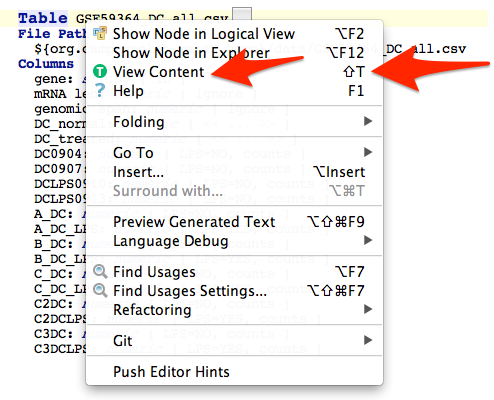
\includegraphics[width=\figWidthNarrow]{figures/ActivateTableViewer.png}
\caption[How to activate the Table Viewer Tool]{\textbf{How to activate the Table Viewer Tool}. The Table Viewer Tool can be activated by right-clicking on the Table and selecting ``View Content'' from the menu. An alternative way is to put the cursor on the Table node and pressing \keys{\shift+T}.}
\label{fig:ActivateTableViewer}
\end{SCfigure}  

\begin{figure}[h!tbp]
  \centering
  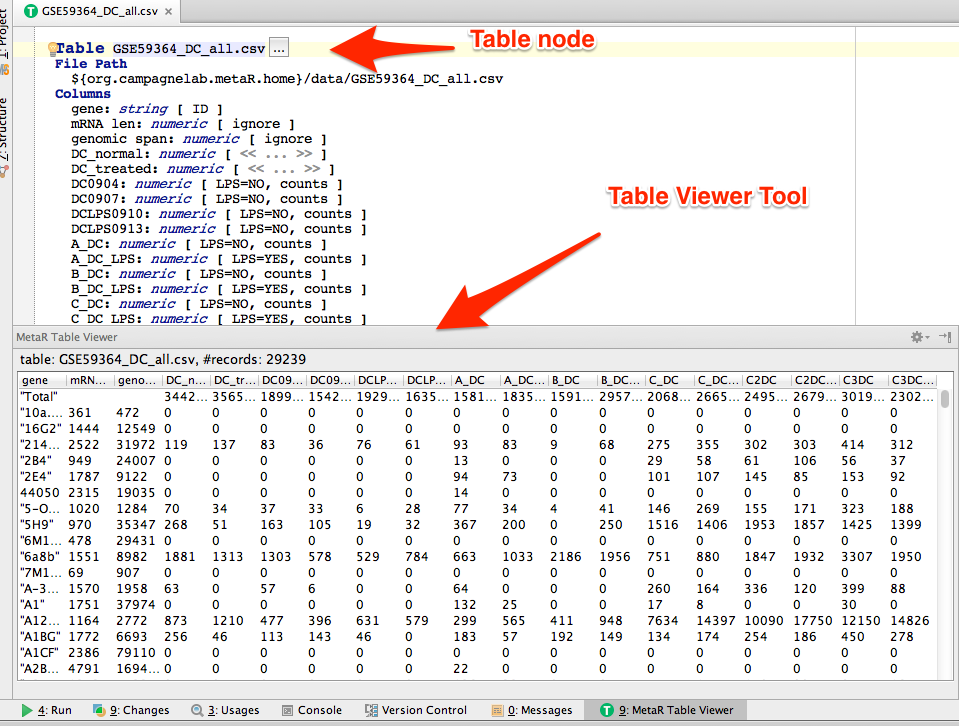
\includegraphics[width=\figWidthWide]{figures/TableViewerInMPS.png}
\caption[The Table Viewer Tool in the MPS UI]{\textbf{The Table Viewer Tool in the MPS UI.} }
\label{fig:TableViewerInMPS}
\end{figure}

\begin{SCfigure}
  \centering
  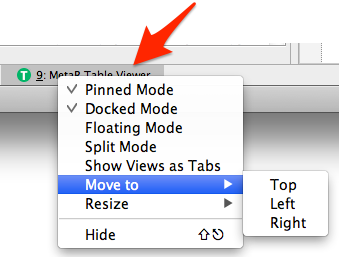
\includegraphics[width=\figWidthTiny]{figures/ToolVisualizationOptions.png}
\caption[Visualization Options for Table Viewer Tool]{\textbf{Visualization Options for Table Viewer Tool}. Different visualization options are available for the Table Viewer Tool. By right clicking on the tool name in the Tool Buttons bar (if not visible, select  \menu{View > Tool Buttons} from the MPS menu), a user can explore them and choose the one that best fits a project needs. In our experience, the floating mode or the Docked/Pinned mode with the panel on the right are very effective.}
\label{fig:ToolVisualizationOptions}
\end{SCfigure}

\begin{figure}[h!tbp]
  \centering
  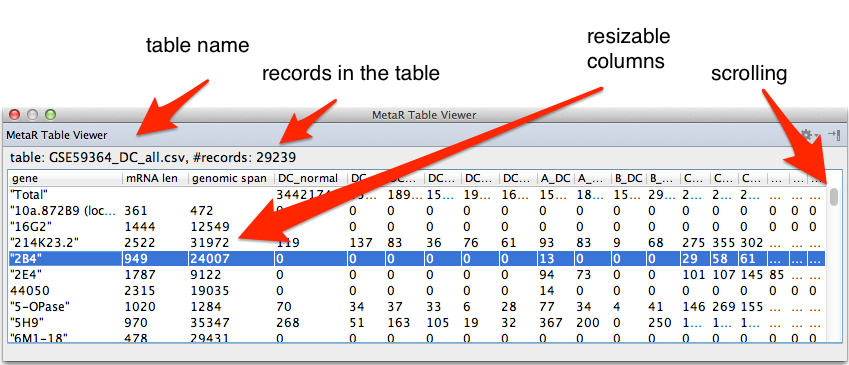
\includegraphics[width=\figWidthWide]{figures/TableViewerToolDetails.png}
\caption[The Table Viewer Tool]{\textbf{The Table Viewer Tool}. The tool displays the content of the selected table. At the top, you can see the name of the table and the number of records loaded. Columns can be resized and rows scrolled for a full visualization of their values.}
\label{fig:ToolVisualizationOptions}
\end{figure}

The tool is immediately available for those tables directly loaded from the file system (e.g. Table nodes) and their references. Other Tables become visible after an Analysis script has been run and the content of the table has been created. In this latter case, the tool is available after the first script execution (see Chapter~\ref{chap:Analyses}). Note that in this case, if the structure and/or content of a table changes, the Analysis script must be executed again before the tool will show the latest table data.


